\chapter{Lösung}
Dieses Kapitel befasst sich mit den Möglichkeiten und Lösungsansätze, zu den Problemstellungen aus Kapitel \ref{ch:problem}. Anhand von Beispielen wird verdeutlicht, wie gewisse Anforderungen umgesetzt werden könnten und wurden.

\section{Meta-Model}
Nach der Anforderungsanalyse, wurden alle relevanten Informationen erkannt und zusammen gestellt. Diese Zusammenstellung an Daten, welche die Applikation beschreiben wird Meta-Model genannt.

\subsection{Kompatibilität mit \acs{gemara} und andern möglichen Clients}

Um die Kompatibilität mit \acf{gemara} zu waren, wurde das Enfield-Meta-Model untersucht. Mit Hilfe dieser Untersuchung konnte festgestellt werden, an welcher Stelle zusätzliche Informationen für die Clients am sinnvollsten eingebaut werden können. So das diese den Ablauf der Applikation gut beschreiben und an den benötigten Stellen alle relevanten Informationen für den Software-Generator zur Verfügung stellt.

Die Abbildung \ref{fig:enfield-model} zeigt die vereinfachte Model-Klasse des Enfield-Meta-Models. 
In dieser Klasse sind bereits die wichtigsten Informationen wie zum Beispiel der Name der Applikation, oder unter welchem Package diese zu finden ist. Neben diesen grundsätzlichen Informationen liefert die Model-Klasse auch den Startpunkt des endlichen Automaten, welcher die Anwendung beschreibt. Dieser Startpunkt ist der \enquote{GetDispatcherState}. Dieses Objekt besitzt das Attribut \enquote{transitions}. Dieses Attribut beschreibt, welche States auf den Dispatcher-State folgen können. Jeder dieser folgenden States, besitzt wiederum eine Collection mit Tansistionen, die auf die nachfolgenden States verweisen. So wird mit Hilfe der Transitionen und der States der endliche Automat der Anwendung beschrieben. Der Generator kann diese Beschreibung nutzen, um zu entscheiden in welcher Reihenfolge, welche Klassen generiert werden müssen.

\begin{figure}[H]
	\begin{center}
		\includegraphics[width=0.86\textwidth]{images/Enfield-Meta-Model.png}
		\caption{Vereinfachter Aufbau des Enfield-Meta-Models}
		\label{fig:enfield-model}
	\end{center}
\end{figure}

Um jetzt zusätzlich benötigten Informationen für die Android Applikation in dieses bestehende Modell einzubauen, gibt es zwei Möglichkeiten.

\subsection{Eigenes Android-Meta-Model}

Es besteht die Möglichkeit die Model-Klasse um ein Attribut \enquote{Android-Meta-Model} zu erweitern.
Die Abbildung \ref{fig:android-model} stellt zeigt schemenhaft ein Beispiel wie ein Android-Meta-Model aussehen könnte. Auffällig hierbei ist das viele Informationen, die das Enfield-Model bereits liefern würde, hier noch einmal explizit beschrieben werden muss. Ein Beispiel wären die Transitionen, zwischen den Fragmenten beziehungsweise zwischen den Activities. 


\begin{figure}[H]
	\begin{center}
		\includegraphics[width=0.86\textwidth]{images/Android-Meta-Model.png}
		\caption{Möglicher Aufbau eines Android-Meta-Models}
		\label{fig:android-model}
	\end{center}
\end{figure}

Der Nutzer des Software-Generators, muss also ziemlich viel über den Ablauf und die Funktionsweiße einer Android-Anwendung wissen, um diesen Generator sinnvoll verwenden zu können.
Dabei bleibt zusätzlich noch die Möglichkeit, das der Nutzer eigens geschriebene Metohden in das Model einpflegen kann. John Abou-Jaoudeh at al., haben in ihrer Arbeit \enquote{A High-Level Modeling Language for Efficent Design, Implementation, and Testing of Android Applications} ein Meta-Model entwickelt, welches genau solche Features unterstützt \cite{abou2015high}.

Der Vorteil einer solchen Erweiterung des Enfield-Models ist, das alle benötigten Daten für die Android Anwendung an einer Stelle zu finden sind. Auch hat der Nutzer die Möglichkeit an manchen Stellen eigene Methoden einzufügen und somit ist er in der Lage das Verhalten der App weiter zu individualisieren.

Jedoch überwiegen in diesem Fall die Nachteile. Ein Nachteil dieses Vorgehens ist, die redundante Beschreibung des Programm-Ablaufes. Einmal im Android-Meta-Model und einmal im Enfield-Meta-Model. Bei jeder Änderung gilt dies zu berücksichtigen. 
Der nächste Nachteil ist der Nutzer des muss sich in der Entwicklung von Android Anwendungen auskennen. Er muss genau das Zusammenspiel von ViewHoldern, Adaptern, Fragments und Activities kennen. Er muss wissen wie diese ineinandergreifen und wann welche Aktionen ausgelöst werden müssen. Weiterhin sollte er ein Grundsätzliches Verständnis für das \acf{mvc} Pattern besitzen, welches bei der Entwicklung von Android Applikationen anwendung findet.
Ein weiterer Nachteil ist die Beschränkung des Models auf Android. Wird das Enfield-Model um ein Android-Meta-Model erweitert, so muss dieses für jeden einzelnen Client geschehen. Soll der Generator beispielsweise um Polymer-Webkomponente oder einer iOS-Anwendung erweitert werden, so müsste für jede einzelne Art von Client, das Enfield-Model mit einem Entsprechenden Meta-Model erweitert werden.

\subsection{Allgemeine Erweiterungen des Enfield-Models an entsprechender Stelle}

In dieser Arbeit wurde sich für die Variante entschieden, das Enfield-Model an ihren \enquote{SingleResourceViews} zu erweitern.
Wird diese Klasse um die  Attribute, die benötigt werden Attribute erweitert, so erhält der Generator die benötigten Ressourcen immer zur rechten Zeit.

Wird beispielsweise eine Instanz eines \enquote{GetPrimarySingleResourceByIdStates} erzeugt, und dessen \enquote{SingleResourceView} enthält alle notwendigen Informationen, um die View in der Android Anwendung zu beschreiben. Kann der Generator mit Hilfe der Transitionen über die States iterieren und verfügt an jedem State über alle benötigten Informationen, um den aktuellen State in der Anwendung generieren zu lassen.

Bei dieser Methode befinden sich alle State-spezifischen Daten direkt am State. Jedoch gibt es neben diesen spezifischen Daten auch Daten, welche die komplette Applikation betreffen, muss das Enfield-Model noch an einer andern Stelle erweitert werden. 
Hierfür erscheint es sinnvoll die Erweiterung direkt in der Model-Klasse vorzunehmen. So kann der Generator schon am Anfang auf diese Daten zugreifen und diese verarbeiten.

Die Abbildung \ref{fig:enfield-model-extended} zeigt das Enfield-Model, welches um die oben genannten Informationen erweitert wurden.

\begin{figure}[H]
	\begin{center}
		\includegraphics[width=0.86\textwidth]{images/Enfield-Meta-Model-Erweitert.png}
		\caption{Vereinfachter Aufbau des erweiterten Enfield-Meta-Models}
		\label{fig:enfield-model-extended}
	\end{center}
\end{figure}

Der Nachteil dieser Methode ist, das die Informationen an mehr als einer Stelle im Enfield-Modell zu finden sind. Sollten die Informationen zu den Clients verändert werden, so sind Änderungen an der SingleResourceView-Klasse und in der Model-Klasse nötig. Die Vorteile wurden jedoch oben schon einmal erwähnt. Der Generator kann das Model als Fahrplan nutzen und weiß genau wann er welche Klassen für die Android Anwendung erzeugen muss. Er kann auch mit Hilfe der Transitionen bestimmen wie der Verlauf innerhalb der Anwendung ablaufen soll.

\subsection{Analyse der benötigten Dateien für das Meta-Model}

Nachdem identifiziert wurde, an welchen Stellen das Enfield-Model erweitert werden soll, muss noch analysiert werden, welche Informationen an diesen Stellen zur Verfügung stehen müssen. Bei dieser Analyse muss auch ein Augenmerk darauf gelegt werden, wie man die Informationen so aufbereitet, dass diese nicht nur eine Android-Applikation, sondern mögliche andere Clients unterstützen.

Die Analyse in dieser Arbeit beschränken sich auf die Clients Android und Polymere-Webkomponente. Bei beiden wird das \acf{ui} nach den Guidelines,des von Google entwickelten Material Design, erstellt \cite{material}. Diese Guidelines schreiben bereits viele nötigen Informationen für die Oberflächengestaltung vor. So wird beispielsweise definiert, das Einträge in einer Liste, als Karte dargestellt werden sollen. Abstände und Icons werden ebenfalls festgelegt.

\subsubsection{CardView}

\begin{figure}[H]
	\begin{center}
		
\includegraphics[width=0.86\textwidth]{images/card.png}
		\caption{Beispiel einer CardView aus einer Liste von Dozenten nach Material Design Guidelines}
		\label{fig:card}
	\end{center}
\end{figure}

\begin{lstlisting}[label=lst:braun_json,
language=json,
firstnumber=1,
caption=Demo Daten eines Dozenten]	
...			   
{
	"address": "Sanderheinrichsleitenweg 20 97074 Wuerzburg",
	"chargeUrl": {
		"href": "https://apistaging.fiw.fhws.de/mig/api/lecturers/4/charges",
		"rel": "chargeUrl",
		"type": "application/vnd.fhws-charge.default+json"
	},
	"email": "peter.braun@fhws.de",
	"firstName": "Peter",
	"homepage": {
		"href": "http://www.welearn.de/.../prof-dr-peter-braun.html",
		"rel": "homepage",
		"type": "text/html"
	},
	"id": 4,
	"lastName": "Braun",
	"phone": "0931/3511-8971",
	"profileImageUrl": {
		"href":"https://apistaging.fiw.fhws.de/.../4/profileimage",
		"rel": "profileImageUrl",
		"type": "image/png"
	},
	"roomNumber": "I.3.27",
	"self": {
		"href": "https://apistaging.fiw.fhws.de/mig/api/lecturers/4",
		"rel": "self",
		"type": "application/vnd.fhws-lecturer.default+json"
	},
	"title": "Prof. Dr."
}
...
\end{lstlisting}

Die  \acf{json} Repräsentation unter Listing \ref{lst:braun_json} beschreibt das Beispiel aus Abbildung \ref{fig:card}.
Jetzt gilt es zu überlegen, wie die Attribute des \ac{json} Objekts aufzubereiten sind, dass diese die Karte des Dozenten widerspiegeln. 

In erster Linie muss entschieden werden, welche der gelieferten Informationen sollen in der Liste für jeden einzelnen Dozenten angezeigt werden. Ist es sinnvoll ist Informationen zu gruppieren? Hier beispielsweise die Attribute \enquote{firstName} und \enquote{lastName}, diese sollen in einer Zeile angezeigt werden. Ist bekannt welche Informationen eine Karte enthalten soll, so muss auch noch die Reihenfolge der einzelnen Attribute der Karte bestimmt werden.
Neben der Reihenfolge gibt es noch die Möglichkeit das die Schriftgröße oder die Schriftfarbe der einzelnen Attribute unterschiedlich sein können. Auch müssen die Standardicons den einzelnen Attribute zuweisen werden. Auch sollte es die möglich sein einzelnen Attribute bestimmte Aktionen zuzuweisen. So sollte beispielsweise beim Klick auf eine Homepage auch diese im Browser geöffnet werden, oder beim Klick auf die Adresse sollte die Applikation Maps öffnen und die angeklickte Adresse dort anzeigen. Gibt es ein Attribut mit dem Hyperlink zu einer Website, sollte es möglich sein einen Text anzugeben, der anstelle des Hyperlinks angezeigt wird. 

Besitzt die Karte ein Bild, so sollte der Nutzer die Möglichkeit besitzen zu entscheiden ob er dieses gerne auf der linken oder der rechten Seite der Karte haben möchte.

\subsubsection{DetailView}

\begin{figure}[H]
	\begin{center}
		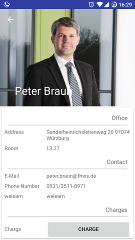
\includegraphics{images/detail.png}
		\caption{Beispiel einer DetailView eines Dozenten nach Material Design Guidelines}
		\label{fig:detail}
	\end{center}
\end{figure}

Die zur Verfügung  stehenden Daten sind die gleichen, welche unter Listing \ref{lst:braun_json} einzusehen sind.

Analog wie bei der CardView stellen Sich auch bei der DetailView, welche Daten alle dargestellt werden sollen. Hier jedoch gibt es zusätzlich zu der horizontalen Gruppierung (Beispiel mit den Vornamen und Nachnamen), auch noch eine vertikale Gruppierung, die im weiteren auch Kategorisierung genannt wird. In der detaillierten Ansicht eines Dozenten gibt es die Möglichkeit die Attribute zu kategorisieren und jeder Kategorie mit einem Namen zu versehen. Für die Gestaltung und Anordnung sowie mögliche Klick-Aktionen müssen die selben Anforderungen wie bei der CardView berücksichtigt werden. 

Jedoch muss die DetailView wissen, welches Attribut den Titel der View darstellt, da dieser in der AppBar erscheinen wird. In diesem Beispiel ist es der Name des Dozenten. Anders als bei der CardView gibt es hier nicht die Möglichkeit zu bestimmen wo das Bild dargestellt werden soll. Ist ein Bild vorhanden, so wird dieses in der Collapsing-Toolbar dargestellt \cite{collapsing}. Andernfalls wird kein Bild angezeigt.

\subsubsection{InputView}

\begin{figure}[H]
	\begin{center}
		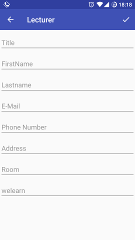
\includegraphics{images/input.png}
		\caption{Beispiel einer View zum Anlegen eines Dozenten}
		\label{fig:input}
	\end{center}
\end{figure}

Für das neu Anlegen eines Dozenten oder auch zum bearbeiten muss entschieden werden, welche Attribute zum Anlegen benötigt werden. Auch hier ist es notwendig die Reihenfolge zu bestimmen. Jedoch kommen in dieser View für jedes Attribut noch die Möglichkeit hinzu ein Hint-Text anzugeben. Dieser Text beschreibt, was in der Android View EditText als Beschreibung für das bestimmte Attribut steht. Weiter sollte es die Möglichkeit geben, jedem Feld eine Nachricht mitzugeben, welche Angezeigt wird, wenn das Feld beispielsweise leer gelassen wird. Oder eine weitere Nachricht, wenn das Eingegebene nicht dem Erwarteten entspricht. Zum Beispiel wurde in das Feld für die E-Mail die Telefonnummer eingegeben. Oder es wurde ein regulärer Ausdruck mitgegeben und das Eingegebene entspricht nicht den Anforderungen, welche durch den regulären Ausdruck definiert wurden.

\subsubsection{Programmablauf und Klick-Aktionen}

Da das Enfield-Model bereits einen endlichen Automaten beschreibt, welcher den Programmablauf widerspiegelt, ist es nicht notwendig, diesen Ablauf noch einmal genauer zu definieren. Da der bereits definierte Ablauf übernommen wird.

Auch die Klick-Aktionen, das Geschehen, welches durch einen Klick auf ein bestimmtes Attribut ausgeführt werden soll, beschränkt sich auf Android Standard Aktionen. Beispielsweise das wechseln zu den Maps, zu einem E-Mail Client, dem Browser oder zum Anrufsmenü. Jede deser Aktion ergibt sich aus den Typen der Attribute, weswegen diese auch nicht weiter definiert werden müssen.

\subsection{Design der View-Meta-Modelle}

In den letzten Abschnitten der Arbeit wurde aufgezählt, was das Meta-Model alles Abdecken muss und das sowohl Android- als auch Polymer-seitig. In diesem Kapitel wird ein Meta-Model vorgestellt, welches die erwähnten Eigenschaften abdeckt.


\begin{figure}[H]
	\begin{center}
		\includegraphics[width=0.86\textwidth]{images/metamodel.png}
		\caption{Aufbau der Views zur Erweiterung des Enfield-Models}
		\label{fig:meta-model}
	\end{center}
\end{figure}

Die Abbildung \ref{fig:meta-model} zeigt den Aufbau der Objekte, mit welchem das Enfield-Model erweitert wird. Die drei Views CardView, DetailView und InputView sind alles Instanzen von AbstraktResourceView. Jede der View, weiß welche Ressource sie darstellen soll. Dies passiert über die Zuordnung mit Hilfe des Ressourcennamens. Die drei Views, lassen sich in zwei Kategorien einteilen: Views, welche Informationen anzeigen und Views welche zur Eingabe von Informationen benötigt werden.
So gehören CardView und DetailView zur anzeigenden Views und die InputView zur zweiten Kategorie. 

\subsubsection{Anzeigende Views}
Diese View-Typen haben die Aufgabe in einer Liste alle Attribute zu halten, welche in der entsprechenden View angezeigt werden sollen. Dabei bestimmt die Reihenfolge, in welcher die Attribute in dieser Liste sind auch die Anordnung in der Oberfläche. Ist das erste Item in der Liste der Name, so wird dieser ganz oben in der View angezeigt.
Bei der DetailView jedoch gibt es nicht eine Liste mit den Attributen, sondern eine Liste mit Kategorien. Diese Kategorien, besitzen 
einen Namen und eine Liste mit den Attributen ihrer Kategorie. Die Darstellungsreihenfolge der Kategorien und deren Attribute ist analog zu der der CardView. Weiter besitzt die DetailView das Attribute \enquote{image}, dieses Attribut wird hier aus der Liste der Attribute herausgezogen, da dieses Attribut bestimmt, ob die View eine Collapsing-Toolbar besitzen wird oder nicht. Wiederum haben beide Views das Attribut \enquote{titleOfResource} dieses bestimmt welches Attribut unserer Ressource beispielsweise in der Toolbar angezeigt wird.

Auf die Polymer-spezifischen Attribute wird in dieser Arbeit nicht weiter eingegangen.

Mit Hilfe der Listen, Titelattributen und dem Bildattribut kann das Erscheinungsbild einer View schon ziemlich gut beschrieben werden. Jetzt bleibt fehlt noch die Möglichkeit, die Schriftgrößen, Schriftfarben, Klick-Aktionen und so weiter zu definieren.
Außerdem ist es bis jetzt nur möglich einfache Attribute anzuzeigen, eine horizontale Gruppierung ist noch nicht möglich. Um diese Anforderungen zu erfüllen, werden nicht Attribute in den Listen gespeichert sondern Ausprägungen von ResourceViewAttributen. 

Es gibt zwei Ausprägungen: ein SingleResourceViewAttribute und ein GroupedResourceViewAttribute.  Das SingleResourceViewAttribute ist für einfache Attribute, mit diesem ist es beispielsweise möglich den Titel eines Dozenten anzuzeigen. Das GroupedresourceViewAttribute ermöglicht die horizontale Gruppierung. Beide Objekte, bestimmen jedoch nicht die Design-spezifischen Eigenschaften des Attributs. Hierfür besitzen beide Attribut-Typen das Attribut DisplayViewAttribute.

Bei der SingleResourceViewAttribute ist diese Instanz von einem AbstractViewAttribute das einzige Attribut, beim GroupedResourceViewAttribute wiederum gibt es eine Liste von diesen DisplayViewAttributen, welche dann die anzuzeigenden Informationen widerspiegeln. Weitergehend besitzt diese Attribut-Art auch noch ein DisplayViewAttribute, welches die neu entstandene Gruppierung beschreiben soll.

Ein DisplayViewAttribute besitzt nun die Möglichkeit, die Schriftgröße und -farbe zu definieren. Die angegebene Farbe muss eine Farbe in hexadezimaler Darstellung sein, wird keine Farbe mitgegeben, wird die Default-Farbe der Anwendung genommen. In der Regel ist diese Schwarz.  Die Schriftgröße wiederum ist auf 3 Stufen beschränkt. Es gibt die Möglichkeit den Text in klein, normal und groß darzustellen. Per default ist normal eingestellt. Aus der Oberklasse AbstractViewAttribute besitzt das DisplayViewAttribute noch die Attribute \enquote{attributeName}, dieses muss exakt so heißen wie in der Definition der Ressource beschrieben.
Mit dem \enquote{attributeLabel} kann angegeben werden, wie dieses Attribut in der View angezeigt werden soll. Die Abbildung \ref{fig:detail} zeigt die Verwendung von den Labels, vor beispielsweise der E-Mailadresse des Dozenten steht \enquote{E-Mail}, dieser String entspricht dem Label des Attributes. Muss angeben werden von welchem Typ das aktuell beschriebene Attribut ist.
Dies geschickt mit dem Attribut AttributeType. Es gibt folgende mögliche Typen: HOME, MAIL, LOCATION, PICTURE, PHONE\_ NUMBER, TEXT, URL, DATE, SUBRESOURCE. Jeder Typ bestimmt die Eigenschaften des Attributes. Über diesen wird bestimmt welches Icon in der Karte vor dem entsprechenden Attribut angezeigt werden. Auch bestimmt er welche Aktion bei Klick ausgeführt werden soll. So wird bei einem Klick auf ein Attribut vom Typ LOCATION versucht die Anwendung Maps zu öffnen und den angezeigten Standort dort anzuzeigen. Ist das Attribute vom Typ SUBRESOURCE so wird für dieses Attribut ein Button angezeigt, dieser ermöglicht es dann zu der entsprechenden Subressource zu wechseln. Diese Klick-Aktionen müssen jedoch mit dem Attribut \enquote{clickActionAndroid} erst aktiviert werden.

Manche Typen bringen noch ein paar andere Besonderheiten mit sich. So muss man beispielsweise bei einem URL-Attribut noch eine Beschreibung mitgeben, welche anstelle der Hyperlinks angezeigt werden soll. Bei einem Bild kann man beispielsweise noch bestimmen, ob dieses links oder rechts dargestellt werden soll. 

In Listing \ref{lst:detailview_impl} ist zu sehen, wie eine DetailView definiert wird.

\begin{lstlisting}[label=lst:detailview_impl,
language=java,
firstnumber=1,
caption=Erstellung einer DetailView]				   
...
DetailView detailView;

try {
List<Category> categories = new ArrayList<>();

DisplayViewAttribute nameAttribute = new DisplayViewAttribute("name", ViewAttribute.AttributeType.TEXT);
GroupResourceViewAttribute name = new GroupResourceViewAttribute(nameAttribute, getViewTitleAttributes());

categories.add(new Category("Office", getOfficeResourceViewAttributes()));
categories.add(new Category("Contact", getContactResourceViewAttributes()));
categories.add(new Category("Charges", getChangeResourceViewAttributes()));

detailView = new DetailView("Lecturer", name, categories);
detailView.setImage(getImage());
} catch (DisplayViewException ex) {
detailView = null;
}
...
private static List<ResourceViewAttribute> getOfficeResourceViewAttributes() {
List<ResourceViewAttribute> officeAttributes = new ArrayList<>();

DisplayViewAttribute addressAttribute = new DisplayViewAttribute("address", ViewAttribute.AttributeType.LOCATION);
addressAttribute.setAttributeLabel("Address");
addressAttribute.setClickActionAndroid(true);
SingleResourceViewAttribute address = new SingleResourceViewAttribute(addressAttribute);
officeAttributes.add(address);

DisplayViewAttribute roomAttribute = new DisplayViewAttribute("roomNumber", ViewAttribute.AttributeType.TEXT);
roomAttribute.setAttributeLabel("Room");
roomAttribute.setClickActionAndroid(true);
SingleResourceViewAttribute room = new SingleResourceViewAttribute(roomAttribute);
officeAttributes.add(room);

return officeAttributes;
}
...
\end{lstlisting}

\subsubsection{Eingebende Views}

Bei der InputView gibt es wieder eine Liste, welche dieses mal InputViewAttribute mit der Oberklasse AbstractViewAttribute hält. Diese Liste bestimmt analog zu den anzeigenden Views die darzustellende Reihenfolge der Attribute. 

Neben dem \enquote{attributeName} der wieder exakt dem Namen aus der Ressourcendefiniton entsprechen muss, besitzt das InputViewAttribute auch die Möglichkeit zu bestimmen, welcher Typ das aktuelle Attribut besitzt. Jedoch haben die Typen hier eine Andere Bedeutung als bei dem anderen View-Typ. So wird beispielsweise bei dem Type DATE kein EditText angezeigt, sondern der Nutzer hat die Möglichkeit das Datum über das DatePicker-Widget von Android einzugeben. 

Es ist jedoch für den Android-Client nicht möglich Bilder zu Ressourcen hinzuzufügen, oder diese zu Bearbeiten. Wird eine Subressource nicht in einer InputView der Oberressource bearbeitet oder neu angelegt. Dies ist dann in der entsprechenden View der Subressource möglich. Die anderen Typen beschränken das EditText-Widget auf die angegebenen Typen. So wird bei einem Klick auf ein PHONE\_NUMBER-Feld die Tastatur im Zahlenmodus ausgefahren und so weiter.

Einem InputViewAttribute muss zusätzlich ein \enquote{hintText} mitgegeben werden, der im EditText des Attributs beschreibt, was in diesem Feld erwartet wird. Mit dem String \enquote{missingText} kann dem Attribut mitgegeben werden, welche Nachricht dem Nutzer angezeigt wird, falls er versucht zu speichern ohne das entsprechende Feld auszufüllen. Mit der Kombination von \enquote{checkPattern} und \enquote{errorText} bekommt der Nutzer des Generators die Validierung des eingegebenen Attributes noch weiter zu verfeinern und auch dem Nutzer der Applikation ein Feedback zu geben, falls eine falsche Eingabe getätigt wurde.

Die Definition einer InputView wird in Listing \ref{lst:inputview_impl} dargestellt.

\begin{lstlisting}[label=lst:inputview_impl,
language=java,
firstnumber=1,
caption=Erstellung einer InputView]				   
...
List<InputViewAttribute> inputViewAttributes = new ArrayList<>();

InputViewAttribute title = new InputViewAttribute("title", ViewAttribute.AttributeType.TEXT, "Title", "Title is missing!");
title.setAttributeLabel("Title");
inputViewAttributes.add(title);

InputViewAttribute firstName = new InputViewAttribute("firstName", ViewAttribute.AttributeType.TEXT, "FirstName",
"Firstname is missing!");
firstName.setAttributeLabel("Firstname");
inputViewAttributes.add(firstName);

InputViewAttribute lastName = new InputViewAttribute("lastName", ViewAttribute.AttributeType.TEXT, "Lastname",
"LastName is missing!");
lastName.setAttributeLabel("Lastname");
inputViewAttributes.add(lastName);

InputViewAttribute mail = new InputViewAttribute("email", ViewAttribute.AttributeType.MAIL, "E-Mail", "E-Mail is missing!");
mail.setAttributeLabel("E-Mail");
inputViewAttributes.add(mail);

InputViewAttribute phone = new InputViewAttribute("phone", ViewAttribute.AttributeType.PHONE_NUMBER, "Phone Number",
"Phone number is missing!");
phone.setAttributeLabel("Phone Number");
inputViewAttributes.add(phone);

InputViewAttribute address = new InputViewAttribute("address", ViewAttribute.AttributeType.TEXT, "Address", "Address is missing!");
address.setAttributeLabel("Address");
inputViewAttributes.add(address);

InputViewAttribute room = new InputViewAttribute("roomNumber", ViewAttribute.AttributeType.TEXT, "Room", "Room is missing!");
room.setAttributeLabel("Room");
inputViewAttributes.add(room);

InputViewAttribute weLearn = new InputViewAttribute("homepage", ViewAttribute.AttributeType.URL, "welearn",
"welearn URL is missing!");
weLearn.setAttributeLabel("welearn");
inputViewAttributes.add(weLearn);

InputView inputView;
try {
inputView = new InputView("Lecturer", inputViewAttributes);
} catch (InputViewException ex) {
inputView = null;
}
...
\end{lstlisting}

\subsection{Analyse und Design von allgemeinen Daten für eine Anwendung}

Dieses Kapitel behandelt die Informationen, welche eine Applikation neben den View-Beschreibungen zusätzlich benötigt, aber diese vom Kontext her nicht in einer der Views beschrieben werden können.

Ein Beispiel für eine solche Information wäre der \acf{url} für den Einstieg. Die Applikation benötigt diesen um zu wissen, unter welcher Adresse sich die anzuzeigenden Informationen zu finden sind. Ein weiteres Beispiel sind die Grundfarben der Applikation. Das Material Design gibt drei benötigte Grundfarben vor: \enquote{colorPrimary}, \enquote{colorprimaryDark} und \enquote{colorAccent} diese Grundfarben wird um die Farbe für den Toolbar-Text erweitert.

Mit dem Wissen, konnte eine Erweiterung des Enfield-Models designed werden, welches in Abbildung \ref{fig:appspecifics} dargestellt ist.

\begin{figure}[H]
	\begin{center}
		\includegraphics[width=0.86\textwidth]{images/appspecifics.png}
		\caption{Aufbau des AppSpecifics-Objekt  zur Erweiterung des Enfield-Models}
		\label{fig:appspecifics}
	\end{center}
\end{figure}

 Über die Map \enquote{additionalInformation} können zusätzlich weitere allgemeine Informationen an den Generator, zur Erzeugung der Anwendung, weitergegeben werden .

\section{Software-Generator}

Nachdem das Meta-Model nun klar ist, geht dieses Kapitel der Ausarbeitung auf die Funktionsweise des Generators ein. 
Es wird dargelegt wie der Generator aufgebaut ist und teilweise darauf eingegangen wieso dieser Weg der Generation gewählt wurde. Des weiteren wird das Java \acf{api} JavaPoet kurz vorgestellt \cite{poet}.

\subsection{JavaPoet}
JavaPoet ist ein Java \ac{api}, welches ermöglicht Java-Klassen zu generieren \cite{poet}. Hierfür wird die zu generierende Klasse programmiert. Mit Hilfe von nur ein paar Schlüsselwörtern ist es recht einfach möglich Klassen, Interfaces oder Methoden zu generieren. 

Da der größte Teil des Generators Java-Klassen erzeugen muss, ist dieses \ac{api} bestens für diesen Zweck geeignet. Sie erspart die aufwändige String-Manipulation. Durch die Nutzung wird auch bei der Ausführung des Programmes sichergestellt, das gültige Konventionen und Regeln eingehalten werden. So ist der grundsätzliche korrekte Aufbau einer Java-Klasse bereits sichergestellt.

Listing \ref{lst:poet} zeigt ein einfaches Beispiel zur Generierung einer Hello-World-Klasse und Listing \ref{lst:poet_result} zeigt das Ergebnis nach der Ausführung des Beispieles.

\begin{lstlisting}[label=lst:poet,
language=java,
firstnumber=1,
caption=Beispiel für die Generation einer Hallo-World-Klasse \cite{poet}]				   
MethodSpec main = MethodSpec.methodBuilder("main")
	.addModifiers(Modifier.PUBLIC, Modifier.STATIC)
	.returns(void.class)
	.addParameter(String[].class, "args")
	.addStatement("$T.out.println($S)", System.class, "Hello, JavaPoet!")
	.build();

TypeSpec helloWorld = TypeSpec.classBuilder("HelloWorld")
	.addModifiers(Modifier.PUBLIC, Modifier.FINAL)
	.addMethod(main)
	.build();

JavaFile javaFile = JavaFile.builder("com.example.helloworld", helloWorld)
	.build();
\end{lstlisting}

\begin{lstlisting}[label=lst:poet_result,
language=java,
firstnumber=1,
caption=Ergebnis der Generation von Listing \ref{lst:poet} \cite{poet}]				   
package com.example.helloworld;

public final class HelloWorld {
	public static void main(String[] args) {
		System.out.println("Hello, JavaPoet!");
	}
}
\end{lstlisting}

\subsection{Generierung anderer Daten-Typen}

Neben Java-Klassen besitzt der Sourcecode einer Android Applikation auch XML-Dateien und Gradle-Dateien. Für diese Typen muss eine andere Möglichkeit der Generierung gewählt werden. Hierfür liefert \acf{gemara} mit der Klasse GeneratedFile eine Möglichkeit. Diese Klasse liefert die die beiden Methoden \enquote{append(String contet)} und \enquote{appendln(String content)}. Welche es ermöglichen jedes beliebige textbasiertes File-Format zu generieren. Ein GeneratedFile Objekt erzeugt eine Datei, welcher mit den beiden erwähnten Methoden Strings hinzugefügt werden können, dies ermöglicht es jede beliebige Textstruktur zu erzeugen. Jedoch liefert diese Klasse keinerlei Validierung, die Datei wird generiert egal ob die Struktur gültig ist oder nicht.

So würde Listing \ref{lst:append} eine Datei \enquote{test.xml} im Verzeichnis \enquote{\\generated} erzeugen. Diese erzeuge Datei wird in Listing \ref{list:append_result} dargestellt.

\begin{lstlisting}[label=lst:append,
language=java,
firstnumber=1,
caption=Beispiel eine GeneratedFile-Instanz zur Erzeugung einer XML-Datei]				   
public class FileGenerator extends GeneratedFile {

	@Override
	public void generate() {
		appendln("<?xml version=\"1.0\" encoding=\"utf-8\"?>");
		appendln("<menu xmlns:android=\"http://schemas.android.com/apk/res/android\" xmlns:app=\"http://schemas.android.com/apk/res-auto\">");
		appendln("<item android:id=\"@+id/saveItem\"");
		appendln("android:title=\"@string/save\"");
		appendln("app:showAsAction=\"always\"\\>");
		appendln("<\\menu>");
	}

	@Override
	protected String getFileName() {
		return "test.xml";
	}

	@Override
	protected String getDirectoryName() {
		return "/generated";
	}
}
\end{lstlisting}

\begin{lstlisting}[label=lst:append_result,
language=xml,
firstnumber=1,
caption=Beispiel für einen Quelltext]				   
<?xml version="1.0" encoding="utf-8"?>
	<menu xmlns:android="http://schemas.android.com/apk/res/android"
		xmlns:app="http://schemas.android.com/apk/res-auto">
		<item android:id="@+id/saveItem"
			android:title="@string/save"
			android:icon="@drawable/ic_done"
			app:showAsAction="always"/>
	</menu>
\end{lstlisting}

\subsection{Aufbau der zu generierenden Applikation}

Um den Generator möglichst zu vereinfachen, ist es hilfreich, eine Referenzimplementierung der gewünschten Applikation mit all ihren Funktionen und Anforderungen zu entwickeln. Bei einer anschließenden Quellcode-Analyse sollte darauf geachtet werden, die einzelnen Klassen soweit zu abstrahieren, das eine Einteilung in generischen und spezifischen Quellcode erfolgen kann. Der generische Quellcode ist einfacher zu generieren, da dieser statisch ist und sich für alle folgenden Implementierungen nicht verändert. Es können auch Überlegungen angestrebt werden, diese generischen Klassen einfach im Generator abzulegen und bei Bedarf zu kopieren. Diese Methode wurde verworfen, da sich andernfalls jedes mal die kopierten Klassen via String-Manipulation bearbeitet werden müssten. Die minimale Änderung welche jedes mal getroffen werden müsste, wäre das Anpassen der Package Anweisung am Anfang der Java-Klassen und die Anpassung der Import-Anweisungen. Eine weitere Überlegung wäre es, diese Klassen in eine Android Bibliothek auszulagern, und diese dann in jede Anwendung zu importieren. Auch von dieser Möglichkeit wurde in der ersten Version abgesehen, da die Applikation bereits aus zwei Komponenten besteht. Der Applikation an sich und einer Bibliothek, welche die Android-Komponenten für die Anwendung enthält. Um die Komplexität zu reduzieren werden die benötigten generischen Klassen als Teil der eingebunden Bibliothek jedes mal aufs neue generiert.

Die Referenzimplementierung für diese Arbeit beinhaltet folgende Features:
\begin{center}
	\begin{tabular}{p{0.4\textwidth}|p{0.4\textwidth}}
		\textbf{Ressource: Dozent} & \textbf{Ressource: Amt} \\ \hline
		\begin{itemize}
			\item Anzeige einer Liste mit Dozenten
			\item Anlegen neuer Dozenten
			\item Anzeigen eines Dozenten in Detail
			\item Bearbeiten eines Dozenten
			\item Löschen eines Dozenten
		\end{itemize}
		&
		\begin{itemize}
			\item Anzeigen einer Liste von Ämtern eines Dozenten
			\item Anlegen neuer Ämter für einen Dozent
			\item Anzeigen eines Amtes eines Dozenten
			\item Bearbeiten eines Amtes eines Dozenten
			\item Löschen eines Amtes eines Dozenten
		\end{itemize}
		\\
	\end{tabular}
\end{center}

Der Aufbau der Referenzimplementierung wird in Abbildung \ref{fig:lecturer} dargestellt. Das Schaubild verdeutlicht das Verhältnis von generischen (weiße Kästen) und spezifischen (rote Kästen) Klassen. Die Anzahl der gleichbleibenden Klassen ist mit etwa 60 Prozent bereits höher als der Anteil an spezifischen Klassen. Je höher der Anteil dieser unveränderlichen Klassen, desto geringer wird die Komplexität des Generators. Da der Aufwand eine spezifische Klasse zu erzeugen mehr Logik benötigt, als eine Klasse, welche immer gleich bleibt.

Daneben zeigt die Abbildung \ref{fig:lecturer} auch noch die Aufteilung der Klassen in Klassen der Applikation (gestrichelte Kästen) und Klassen der Bibliothek (solide Kästen). Die Applikation an sich besteht nur aus ein paar wenigen Fragmenten und Aktivities, welche alle projektspezifisch sind. Der komplette generische Quellcode befindet sich in der Bibliothek. Des weiteren befinden sich dort auch die spezifischen Komponenten, beispielsweise der \enquote{LecturerInputView}. Diese Komponente, kann in den Fragmenten zur Bearbeitung oder Neuanlage eines Dozenten dann mit wenigen Zeilen Programmcode verwendet werden.

Diese Art der Aufteilung ermöglicht es das ein Applikation Entwickler sich die Komponente, für das Anzeigen, Bearbeiten, Löschen und der Neuanlage generieren lassen kann. Diese Komponenten jedoch beliebig in seiner eigenen Applikation verwenden kann.

\begin{figure}[H]
	\begin{center}
		\includegraphics[width=\textwidth]{images/Lecturer.png}
		\caption{Aufbau der Referenzimplementierung}
		\label{fig:lecturer}
	\end{center}
\end{figure}

\subsection{Aufbau des Generators}


\begin{figure}[H]
	\begin{center}
		\includegraphics[width=\textwidth]{images/Welling.png}
		\caption{Aufbau des Android-Generators Welling}
		\label{fig:welling}
	\end{center}
\end{figure}




\begin{lstlisting}[label=lst:java,
				   language=java,
				   firstnumber=1,
				   caption=Beispiel für einen Quelltext]				   

public void foo() {				   
	// Kommentar
}
\end{lstlisting}

Lorem ipsum dolor sit amet, consectetur adipiscing elit. Ut vehicula felis lectus, nec aliquet arcu aliquam vitae. Quisque laoreet consequat ante, eget pretium quam hendrerit at. Pellentesque nec purus eget erat mattis varius. Nullam ut vulputate velit. Suspendisse in dui in eros iaculis tempus. Phasellus vel est arcu. Vestibulum ante ipsum primis in faucibus orci luctus et ultrices posuere cubilia Curae; Integer elementum, nulla eu faucibus dignissim, orci justo imperdiet lorem, luctus consectetur orci orci a nunc.

Praesent at nunc nec tortor viverra viverra. Morbi in feugiat lectus. Vestibulum iaculis ipsum at eros viverra volutpat in id ipsum. Donec condimentum, ligula viverra pharetra tincidunt, nunc dui malesuada nisi, vitae mollis lacus massa quis velit. Integer feugiat ipsum a volutpat scelerisque. Nulla facilisis augue nunc. Curabitur eget consectetur nulla. Integer accumsan sem non nisi tristique dictum.

Sed lacinia eu dolor sed congue. Ut dui orci, venenatis id interdum rhoncus, mattis elementum massa. Proin venenatis elementum purus ut rutrum. Phasellus sit amet enim porta, commodo mauris a, bibendum tortor. Nulla ut lobortis justo. Aenean auctor mi nec velit fermentum, quis ultricies odio viverra. Maecenas ultrices urna vel erat ornare, quis suscipit odio molestie. Donec vel dapibus orci, vel tincidunt orci.

Etiam vitae eros erat. Praesent nec accumsan turpis, et mollis eros. Praesent lacinia nulla at neque porta aliquam. Quisque elementum neque ac porta suscipit. Nulla volutpat luctus venenatis. Aliquam imperdiet suscipit pretium. Nunc feugiat lacinia aliquet. Mauris ut sapien nec risus porttitor bibendum. Aenean feugiat bibendum lectus, id mattis elit adipiscing at. Pellentesque interdum felis non risus iaculis euismod fermentum nec urna. Nullam lacinia suscipit erat ac ullamcorper. Sed vitae nulla posuere, posuere sem id, ultricies urna. Maecenas eros lorem, tempus non nulla vitae, ullamcorper egestas nibh. Vestibulum facilisis ante vel purus accumsan mattis. Donec molestie tempor eros, a gravida odio congue posuere.

Sed in tempus elit, sit amet suscipit quam. Ut suscipit dictum molestie. Etiam quis porta mauris. Cras dapibus sapien eget sem porta, ut congue sapien accumsan. Maecenas hendrerit lobortis mauris ut hendrerit. Suspendisse at aliquet est. Quisque eros est, scelerisque ac orci quis, placerat suscipit lorem. Phasellus rutrum enim non odio ullamcorper, sit amet auctor nulla fringilla. Nunc eleifend vulputate dui, a sollicitudin tellus venenatis non. Cras condimentum lorem at ultricies vestibulum. Vestibulum interdum lobortis commodo. Nullam rhoncus interdum massa, ut varius nisi scelerisque id. Nunc interdum quam in enim bibendum vulputate.